%% This is an example first chapter.  You should put chapter/appendix that you
%% write into a separate file, and add a line \include{yourfilename} to
%% main.tex, where `yourfilename.tex' is the name of the chapter/appendix file.
%% You can process specific files by typing their names in at the 
%% \files=
%% prompt when you run the file main.tex through LaTeX.
\chapter{Pendahuluan}

\section{Apa Itu Ijah Webserver?}

	\subsection{Definisi}
	Ijah Webserver merupakan sebuah webserver yang menyajikan pencarian dan/atau prediksi terhadap hubungan antara tanaman dan khasiatnya pada suatu penyakit. Informasi yang disajikan berupa hubungan antara tanaman dengan senyawa (Plant-Compound), senyawa dengan bioprotein (Compound-Protein), dan bioprotein dengan penyakit (Protein-Disease). Selain pencarian dari \emph{database}, Ijah juga melakukan prediksi terhadap hubungan yang belum diketahui menggunakan beberapa jenis algoritme, dan memberikan hasil berupa tingkat kemungkinan kebenaran prediksi. Hasil keterhubungan ini (baik hasil pencarian maupun prediksi) disajikan dalam beberapa jenis keluaran, yang utama yaitu visualisasi dalam bentuk graf \emph{multi-partite}. Tujuan Ijah Webserver adalah menyederhanakan dan membantu proses penelitian obat herbal atau Jamu dengan memberikan informasi potensi tanaman.

	\subsection{Kasus-penggunaan \emph{(use-case)}}
	Ada beberapa kasus-penggunaan \emph{(use-case)} dalam pencarian saat menggunakan Ijah Webserver.
		\subsubsection{Use-case 1 (Both drug-and-target inputs)} \label{sssec:end to end}
		\emph{Use-case} ini melibatkan kedua sisi input yaitu \emph{Drug-side} dan \emph{Target-side}. pada \emph{use case} ini, input dari kedua sisi harus ada. Pencarian ini bersifat end-to-end, misalkan Plant to Disease, dimana kita memasukkan beberapa jenis tanaman dari sisi Drug-side dan beberapa jenis penyakit dari Target-side, lalu hasilnya akan menunjukkan senyawa apa dalam tanaman tersebut yang dapat menarget protein yang ada dalam penyakit tersebut, sehingga berkhasiat menyembuhkan. Variasi input pada \emph{use-case} ini meliputi \textbf{Plant-Protein}, \textbf{Plant-Disease}, \textbf{Compound-Protein}, dan \textbf{Compound-Disease}.
		\subsubsection{Use-case 2 (Drug-side inputs only)} \label{sssec:drug only}
		\emph{Use-case} ini melibatkan hanya satu sisi yaitu \emph{Drug-side} saja. pada \emph{use-case} ini, input dari salah satu \emph{drug-side} (Plant atau Compound) harus ada. Sifat pencarian ini, misal kita memasukkan tanaman saja (Plant Search Only), maka semua senyawa yang terkandung dalam tanaman itu akan muncul, lalu protein yang terkait dengan senyawa tersebut, dan penyakit yang terkait dengan protein tersebut. Sederhananya semua yang terkait dengan tanaman yang diinputkan. Variasi input pada \emph{use-case} ini meliputi \textbf{Plant Search Only} dan \textbf{Compound Search Only} yang pada dasarnya sama dengan Plant Search.
		\subsubsection{Use-case 3 (Target-side inputs only)} \label{sssec:target only}
		\emph{Use case} ini melibatkan hanya satu sisi yaitu \emph{Target-side} saja. pada \emph{use case} ini, input dari salah satu \emph{Target-side} (Protein atau Disease) harus ada. Sifat pencarian ini mirip dengan Drug inputs only, namun bedanya dari sisi Target. Misal pada pencarian dari penyakit (Disease Search Only) akan muncul semua yang berkaitan dengan penyakit itu, termasuk tanaman yang berhubungan. Variasi input pada \emph{use-case} ini meliputi \textbf{Protein Search Only} dan \textbf{Disease Search Only}.


	\subsection{Menu-menu} %brief description about the menus
	Pada Ijah Webserver sendiri terdapat beberapa menu yang bisa dipilih:
	\begin{itemize}
	\item Home
	\item Manual
	\item Downloads
	\item Help/FAQ
	\item IjahV1
	\item Disclaimer
	\item ContactUs
	\item AboutUs
	\end{itemize}
	Penjelasan tentang menu-menu ini ada pada bagian \textbf{\nameref{chap:Menu}}


\section{Tampilan Awal \emph{(Home Page)}}
	 
	\subsection{Overview}
		\subsubsection{URL} \label{ssec:URL ijah}
		Ijah Webserver dapat diakses pada alamat URL \href{http://ijah.apps.cs.ipb.ac.id}{\textbf{http://ijah.apps.cs.ipb.ac.id}}

		\subsubsection{Home Page} %view home + penunjuk bagian
		
		\begin{figure}[!h]
		\centering
		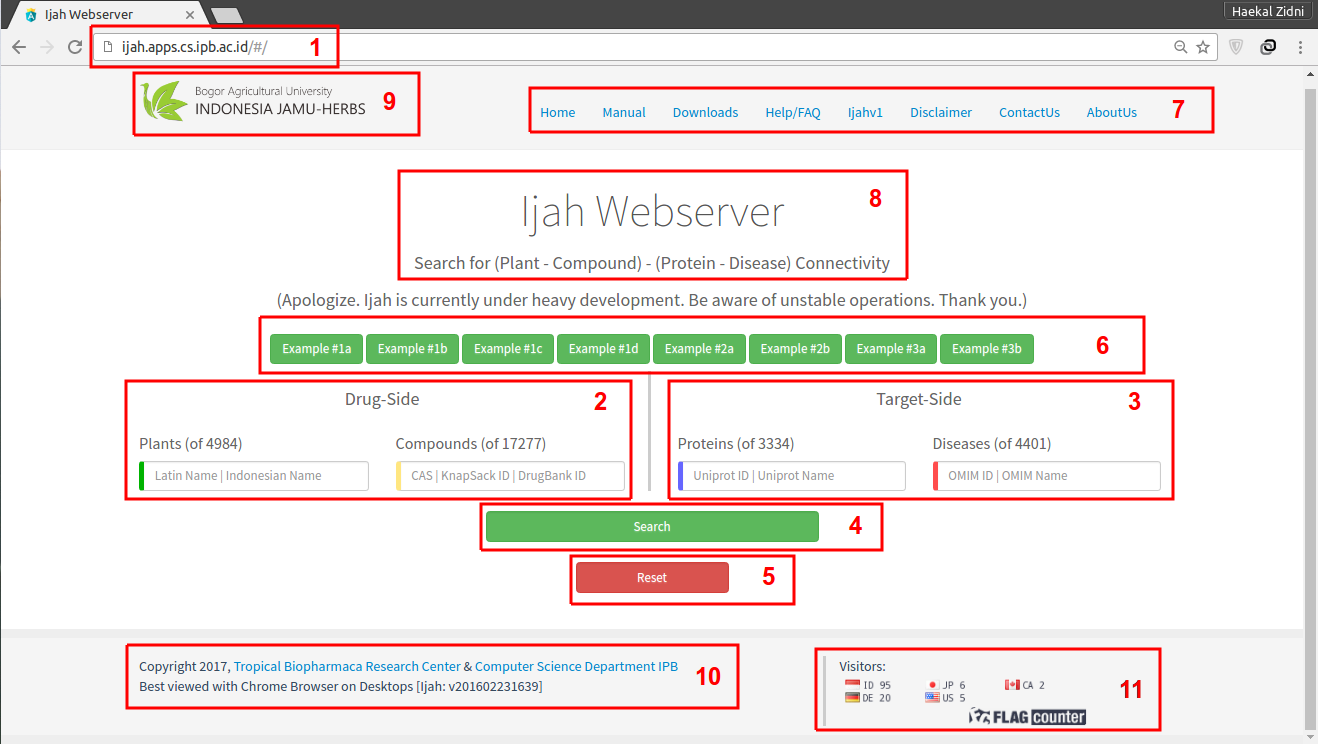
\includegraphics[scale=0.3]{ijah_home_overview.png}
		\caption{Halaman utama Ijah Webserver:
		(1) \hyperref[ssec:URL ijah]{URL Ijah};
		(2) \hyperref[sssec:drug input]{Kotak Masukan \emph{Drug-side}};
		(3) \hyperref[sssec:target input]{Kotak Masukan \emph{Target-side}};
		(4) \hyperref[sssec:search]{Tombol Eksekusi (Search/Search and Predict)};
		(5) \hyperref[sssec:reset]{Tombol Reset};
		(6) \hyperref[ssec:example button]{Deretan Tombol Contoh};
		(7) \hyperref[ssec:menu list]{Deretan Menu};
		(8) \hyperref[ssec:judul]{Judul};
		(9) \hyperref[ssec:judul]{Logo Ijah Webserver};
		(10) \hyperref[ssec:judul]{\emph{Copyright} dan versi Ijah};
		(11) \hyperref[ssec:visitor log]{\emph{Visitor Log}}}
		\label{fig:ijah_home_overview}
		\end{figure}

	\subsection{Kotak Masukan \emph{(Input Fields)}}
		\subsubsection{Drug-side} \label{sssec:drug input}
		Pada Drug-side, input terdiri dari tanaman (Plant) dan senyawa (Compound). Untuk menjaga konsistensi, ketika salah satu dipilih, maka pilihan lain akan menghilang, misal kita telah memilih untuk menginputkan Plant, maka Compound tidak bisa dipilih, begitu pula sebaliknya. Jika ingin mengembalikan/mengosongkan kondisi input kembali, gunakan tombol \hyperref[reset]{\textbf{Reset}}.
			\paragraph{Plants}
			Input Plant terdiri dari nama Latin dan nama Indonesia dari tanaman, yang dipisahkan oleh suatu garis vertikal. Hal ini memudahkan jika kita hanya mengetahui nama latin suatu tanaman dan tidak mengetahui nama lokalnya, begitu pula sebaliknya jika hanya mengetahui nama lokalnya. Selain membantu pencarian, pada kasus salah satu nama tidak diketahui maka akan didapat pengetahuan mengenai nama tanaman tersebut.
			\paragraph{Compounds}
			Input Compound terdiri dari ID CAS, \hyperref[pubchem]{ID PubChem}, atau nama IUPAC dari senyawa tersebut, setiap ID dipisahkan oleh garis vertikal. 
		\subsubsection{Target-side} \label{sssec:target input}
		Pada Target-side, input terdiri dari Protein dan penyakit (Disease). Untuk menjaga konsistensi, ketika salah satu dipilih, maka pilihan lain akan menghilang, misal kita telah memilih untuk menginputkan Protein, maka Disease tidak bisa dipilih, begitu pula sebaliknya. Jika ingin mengembalikan/mengosongkan kondisi input kembali, gunakan tombol \hyperref[reset]{\textbf{Reset}}.
			\paragraph{Protein}
			Input Protein terdiri dari \hyperref[uniprot]{nama Uniprot, singkatan \emph{abbreviation} Uniprot, atau ID Uniprot}. Nama dan ID dipisahkan oleh garis vertikal.
			\paragraph{Disease}
			Input Disease terdiri dari \hyperref[omim]{nama OMIM atau ID OMIM}. Nama dan ID dipisahkan oleh garis vertikal.

	\subsection{Tombol Eksekusi}
	Setelah memberikan input, ada beberapa aksi yang dapat dilakukan, yaitu meneruskan pencarian dengan tombol Search atau mengosongkan semua input dengan tombol Reset.
		\subsubsection{Search (Search and Predict)} \label{sssec:search}
		Bergantung pada jenis input yang diberikan, tombol ini dapat menjalankan fungsi Search saja atau Search and Predict. Lengkapnya lihat pada bagian \hyperref[process]{\textbf{Proses}}.
		\subsubsection{Reset} \label{sssec:reset}
		Tombol Reset ini \textbf{memiliki fungsi yang cukup penting}. Saat ini terdapat kekurangan dimana saat menghapus input, input tidak benar-benar terhapus namun telah tersimpan untuk diproses. Sementara kekurangan ini masih diusahakan untuk diatasi, \textbf{\emph{sangat dianjurkan}} menggunakan tombol Reset ini untuk menghapus input ke kondisi kosong semula.

	\subsection{Deretan Tombol Contoh \emph{(Example)}} \label{ssec:example button}
	Deretan tombol contoh ini merupakan kumpulan contoh \emph{use-case} yang ada pada Ijah Webserver. Jadi selain menggunakan input manual, tombol-tombol contoh ini dapat memudahkan dalam menuju \emph{use-case} tertentu. Kumpulan contoh ini terbagi menjadi tiga kelompok, dimana Example \#1a - \#1d merupakan \emph{use-case} \hyperref[end to end]{\emph{Both Drug and Target inputs}}, Example \#2a - \#2b merupakan \emph{use-case} \hyperref[drug only]{\emph{Drug inputs only}}, dan Example \#3a - \#3b merupakan \emph{use-case} \hyperref[target only]{\emph{Target inputs only}}. Lebih lengkapnya:

	\begin{itemize}
	\item \textbf{Example \#1a} - Plant-Disease
	\item \textbf{Example \#1b} - Plant-Protein
	\item \textbf{Example \#1c} - Compound-Protein
	\item \textbf{Example \#1d} - Compound-Disease
	\item \textbf{Example \#2a} - Plant search only
	\item \textbf{Example \#2b} - Compound search only
	\item \textbf{Example \#3a} - Protein search only
	\item \textbf{Example \#3b} - Disease search only
	\end{itemize}

	\subsection{Deretan Menu} \label{ssec:menu list}
	Pada bagian ini ada sederetan menu yang dapat di-klik. Penjelasan lebih lanjut tentang menu ini ada pada bagian \textbf{\nameref{Menu}}.

	\subsection{Judul, Versi, Logo, dan \emph{Copyright} Ijah} \label{ssec:judul}
	Pada bagian tengah halaman terdapat judul webserver ini, yaitu \textbf{``Ijah Webserver -- Search for (Plant-Compound) -- (Protein-Disease) Connectivity''}. Logo Ijah terdapat pada bagian kiri atas. Pada bagian bawah kiri halaman terdapat bagian yang berisi \emph{copyright} dan versi Ijah Webserver yang berjalan. Di bagian ini juga ada saran penggunaan untuk pengalaman terbaik saat menggunakan Ijah Webserver. Pada nomor versi Ijah Webserver, 8 digit pertama merupakan format tahun-bulan-tanggal dan 4 digit terakhir merupakan jam dan menit. Sebagai contoh di Ijah Webserver v201702231639 berarti versi ini di-\emph{deploy} pada tanggal 23 Februari 2017 pukul 16:39. Pada \emph{copyright} dijelaskan bahwa hak cipta Ijah Webserver ada pada Departemen Ilmu Komputer IPB dan Pusat Riset Biofarmaka IPB.


	\subsection{Visitor Log} \label{ssec:visitor log}
	Visitor Log terdapat di sebelah kanan bawah, setelah \emph{copyright} dan versi. Visitor Log adalah fitur yang menghitung jumlah kunjungan Ijah Webserver beserta negara asal kunjungan. Area Visitor Log ini dapat diklik untuk melihat statistik kunjungan lebih lengkap, seperti pada gambar \ref{fig:ijah_flagcount}

	\begin{figure}[H]
	\centering
	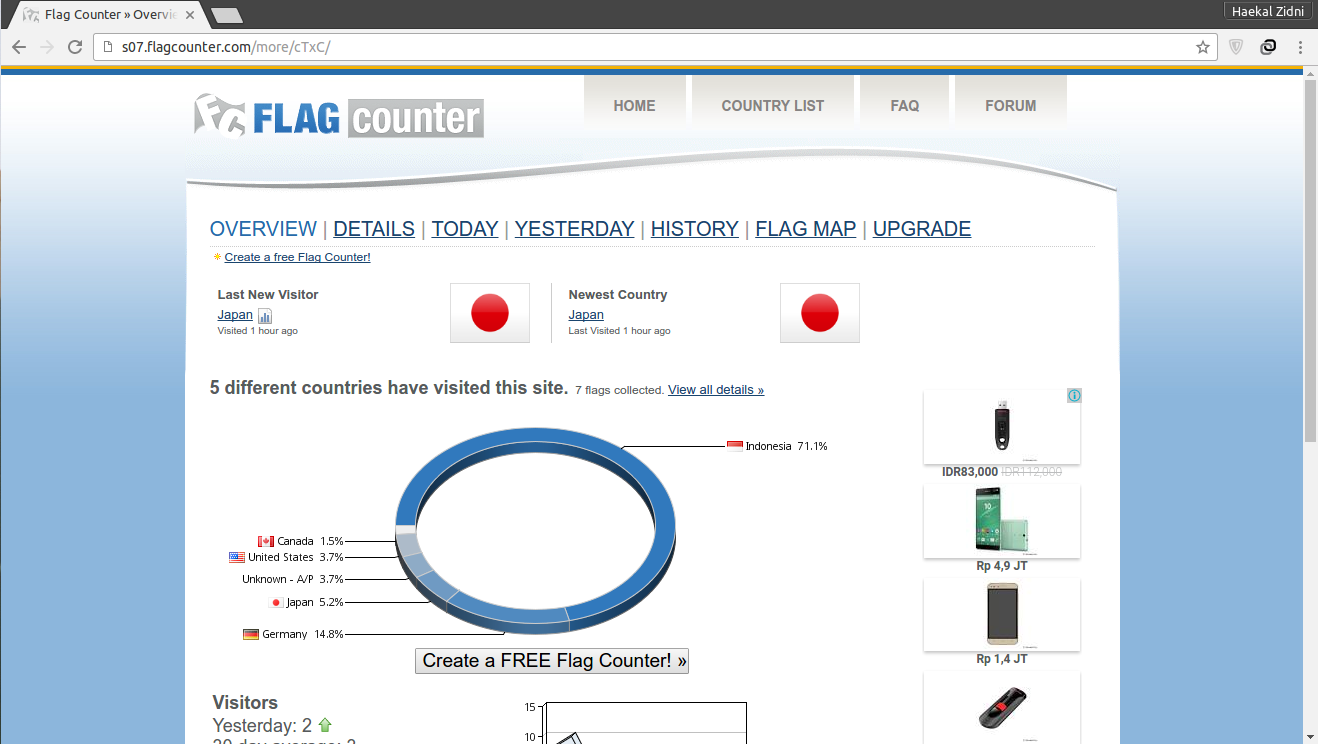
\includegraphics[scale=0.3]{ijah_flagcount.png}
	\caption{Statistik lebih detail yang akan muncul setelah mengklik area Visitor Log}
	\label{fig:ijah_flagcount}
	\end{figure}

\section{Repositori \emph{Source Code}} \label{sec:ws_source}
\emph{Source Code} untuk Ijah Webserver dapat diakses di repositori GitHub di alamat URL \href{https://github.com/tttor/csipb-jamu-prj}{\textbf{https://github.com/tttor/csipb-jamu-prj}}.

Pada repositori ini terdapat beberapa folder untuk setiap \emph{source code}

\begin{itemize}
\item \textbf{Webserver}\\
\href{https://github.com/tttor/csipb-jamu-prj/tree/master/webserver}{\textbf{https://github.com/tttor/csipb-jamu-prj/tree/master/webserver}}.
\item \textbf{Predictor}\\
\href{https://github.com/tttor/csipb-jamu-prj/tree/master/predictor}{\textbf{https://github.com/tttor/csipb-jamu-prj/tree/master/predictor}}.
\item \textbf{Database} (lihat bab \ref{db chapter} )\\
\href{https://github.com/tttor/csipb-jamu-prj/tree/master/database}{\textbf{https://github.com/tttor/csipb-jamu-prj/tree/master/database}}.
\end{itemize}
